\section{Results}
\label{sec:results}
  \begin{table*}
    \centering
    \resizebox{\linewidth}{!}{
      \begin{tabular}{l|ccc@{}|ccc@{}|ccc@{}|ccc@{~}}
        \toprule
        \multirow{2}{*}{\textbf{Method}} & \multicolumn{3}{c|}{\textbf{Linguistics}} & \multicolumn{3}{c|}{\textbf{Archaeology}} & \multicolumn{3}{c|}{\textbf{DUC}} & \multicolumn{3}{c}{\textbf{SemEval}}\\
        \cline{2-13}
        & P & R & F$^{~~~~}$ & P & R & F$^{~~~~}$ & P & R & F$^{~~~~}$ & P & R & F$^{~~}$\\
        \hline
        TopicRank & 11.3 & 13.1 & 12.0$^{~~~~}$ & 28.1 & 19.1 & 22.2$^{~~~~}$ & 17.8 & 22.7 & 19.7$^{~~~~}$ & 14.6 & 10.1 & 11.8$^{\ddagger}$\\
        KEA++ & 11.6 & 13.0 & 12.1$^{\dagger~~}$ & 23.5 & 16.2 & 18.8$^{~~~~}$ & --- & --- & ---$^{~~~~}$ & --- & --- & ---\\
        \hline
        TopicCoRank$_\textnormal{\textit{extr}}$ & 14.6 & 16.8 & 15.4$^{\dagger~~}$ & 36.4 & 24.6 & 28.7$^{~~~~}$ & 25.5 & 32.4 & 28.1$^{\dagger~~}$ & 15.2 & 10.6 & 12.4$^{\ddagger}$\\
        TopicCoRank$_\textnormal{\textit{assign}}$ & \textbf{24.9} & \textbf{28.9} & \textbf{26.4$^{\dagger\ddagger}$} & \textbf{49.1} & \textbf{33.3} & \textbf{38.8}$^{~~~~}$ & 25.9 & 33.3 & 28.8$^{\dagger~~}$ & 11.6 & ~~8.3 & ~~9.5$^{~~}$\\
        \hline
        TopicCoRank & 19.0 & 22.0 & 20.1$^{\dagger~~}$ & 39.5 & 26.6 & 31.1$^{~~~~}$ & \textbf{28.4} & \textbf{36.6} & \textbf{31.5$^{\dagger\ddagger}$} & \textbf{16.4} & \textbf{11.6} & \textbf{13.4$^{\ddagger}$}\\
        \bottomrule
      \end{tabular}
    }
    \caption{Comparison of TopicCoRank with the baselines. Precision (P), Recall
             (R) and F-score (F) are reported in percentages. $\dagger$ and $\ddagger$
             indicate a significant F-score improvement over, respectively, TopicRank and
             KEA++. \TODO{T-Test with KEA++}
             \label{tab:comparison_results}}
  \end{table*}
  Table~\ref{tab:comparison_results} summarizes the performance for three datasets of TopicCoRank,  TopicRank, and \textit{Assignment}, the keyphrase assignment baseline.
  The results show that \textit{Assignment} performs better than TopicRank on Inist and DUC datasets, to the contrary of
  SemEval. 
  %Results show the necessity, in some cases, to perform keyphrase assignment over keyphrase extraction.
  Keyphrase assignment seems to be more appropriate than keyphrase extraction for Inist and DUC text collections.
  %Based on observations from table~\ref{tab:corpus_statistics},  heterogeneously annotated are more difficult to treat by keyphrase assignment methods.
  Keyphrase extraction has to be preferred to keyphrase assignment for datasets such as SemEval that was heterogeneously annotated. 
  The main result is that TopicCoRank outperforms both TopicRank and \textit{Assignment} on all
  datasets. 
  
  Table~\ref{tab:comparison_results} shows the performance of two variants of TopicCoRank: TopicCoRank$_\textnormal{\textit{extr}}$ performs only  extraction
  and  TopicCoRank$_\textnormal{\textit{assign}}$ only assignment.
  The results of TopicCoRank$_\textnormal{\textit{extr}}$ and 
  TopicCoRank$_\textnormal{\textit{assign}}$ confirm that keyphrase assignment is more appropriate for 
  Inist and DUC, whereas keyphrase extraction is for SemEval.
  TopicCoRank outperforms TopicCoRank$_\textnormal{\textit{extr}}$ for all datasets.
  TopicCoRank outperforms TopicCoRank$_\textnormal{\textit{assign}}$ on DUC and SemEval, but not on Inist.
  
  %Inist contains so much missing keyphrases that domain keyphrases must be prioritized over document topics. 
  The Inist keyphrases are mainly missing keyphrases, i.e., domain keyphrases that do not occur in the bibliographic records. 
  For such dataset, domain keyphrases need to be prioritized over document topics. This could be done by giving more weight to the outer recommendation during the graph-based co-ranking.
  
  TopicCoRank and TopicCoRank$_\textnormal{\textit{extr}}$ outperform TopicCoRank$_\textnormal{\textit{assign}}$ for DUC and SemEval.
  The graph co-ranking algorithm successfully leverages document topics and
  controlled keyphrases to output both new concepts and appropriate controlled keyphrases.
  The new concepts that are identified could be used further to update domain-specific terminology.

  \ANNOTATE{Table~\ref{tab:assignment_ratio} shows the percentage of assigned keyphrases by TopicCoRank
  for each dataset. The statistics show that the co-ranking actually works and outputs both
  domain keyphrases and keyphrases from the document independently.}{Strengthen}
  \begin{table}[!h]
    \centering
    \begin{tabular}{l|c}
        \toprule
        & Assignment ratio\\
        \hline
        Linguistics & 38.7\%\\
        Archaeology & 32.2\%\\
        DUC & 58.6\%\\
        SemEval & 40.0\%\\
        \bottomrule
    \end{tabular}
    \caption{Percentage of assignment performed by TopicCoRank for 10 keyphrases
             \label{tab:assignment_ratio}}
  \end{table}
  
  To get a better understanding of the performance of each method, we plot
  precision-recall curves. Figure~\ref{fig:pr_curves1} shows the precision-recall curves
  of TopicRank, \textit{Assignment} and TopicCoRank for each dataset. 
  %Again, we can see that TopicCoRank outperforms the baselines. 
  TopicCoRank and TopicRank %have the same behavior. 
  behave similarly.  TopicCoRank is boosted by the keyphrase assignment. It achieves a better
  maximum precision and a better maximum recall.
  %boosted by keyphrase assignment. %Figure~\ref{fig:pr_curves2} shows the precision-recall
  %curves of TopicCoRank$_\textnormal{\textit{extr}}$,
  %TopicCoRank$_\textnormal{\textit{assign}}$ and TopicCoRank for each dataset. \TODO{\dots}
  \begin{figure*}
      \centering
      \subfigure[Linguistics]{
        \begin{tikzpicture}[every axis/.append style={font=\footnotesize}]
          \pgfkeys{/pgf/number format/.cd, fixed}
          \begin{axis}[x=0.0076038\linewidth,
                       xtick={0, 20, 40, ..., 100},
                       xmin=0,
                       xmax=40,
                       xlabel=recall (\%),
                       x label style={yshift=.34em},
                       y=0.0076038\linewidth,
                       ytick={0, 10, 20, ..., 100},
                       ymin=0,
                       ymax=40,
                       ylabel=precision (\%),
                       y label style={yshift=-1.1em},
                       legend style={font=\footnotesize}]
            \addplot [red, mark=+] file {input/data/linguistique_topicrank.csv};
            \addplot [green, mark=-] file {input/data/linguistique_kea_pp.csv};
            \addplot [blue, mark=x] file {input/data/linguistique_topiccorank.csv};
            \addplot [dotted, domain=20:40] {(30 * x) / ((2 * x) - 30)};
            \addplot [dotted, domain=10:40] {(20 * x) / ((2 * x) - 20)};
            \addplot [dotted, domain=5:40] {(10 * x) / ((2 * x) - 10)};
            \legend{TopicRank, KEA++, TopicCoRank};
          \end{axis}
          \node at (4.9,3.1) [anchor=east] {\footnotesize{F=0.30}};
          \node at (4.9,1.8) [anchor=east] {\footnotesize{F=0.20}};
          \node at (4.9,0.9) [anchor=east] {\footnotesize{F=0.10}};
        \end{tikzpicture}
      }
      \subfigure[Archaeology]{
        \begin{tikzpicture}[every axis/.append style={font=\footnotesize}]
          \pgfkeys{/pgf/number format/.cd, fixed}
          \begin{axis}[x=0.0050692\linewidth,
                       xtick={0, 20, 40, ..., 100},
                       xmin=0,
                       xmax=60,
                       xlabel=recall (\%),
                       x label style={yshift=.34em},
                       y=0.0050692\linewidth,
                       ytick={0, 15, 30, ..., 100},
                       ymin=0,
                       ymax=60,
                       ylabel=precision (\%),
                       y label style={yshift=-1.1em},
                       legend style={font=\footnotesize}]
            \addplot [red, mark=+] file {input/data/archeologie_topicrank.csv};
            \addplot [green, mark=-] file {input/data/archeologie_kea_pp.csv};
            \addplot [blue, mark=x] file {input/data/archeologie_topiccorank.csv};
            \addplot [dotted, domain=30:60] {(40 * x) / ((2 * x) - 40)};
            \addplot [dotted, domain=20:60] {(30 * x) / ((2 * x) - 30)};
            \addplot [dotted, domain=10:60] {(20 * x) / ((2 * x) - 20)};
            \addplot [dotted, domain=5:60] {(10 * x) / ((2 * x) - 10)};
            \legend{TopicRank, KEA++, TopicCoRank};
          \end{axis}
          \node at (4.9,2.65) [anchor=east] {\footnotesize{F=0.40}};
          \node at (4.9,1.85) [anchor=east] {\footnotesize{F=0.30}};
          \node at (4.9,1.15) [anchor=east] {\footnotesize{F=0.20}};
          \node at (4.9,0.65) [anchor=east] {\footnotesize{F=0.10}};
        \end{tikzpicture}
      }
      \subfigure[DUC]{
        \begin{tikzpicture}[every axis/.append style={font=\footnotesize}]
          \pgfkeys{/pgf/number format/.cd, fixed}
          \begin{axis}[x=0.0050692\linewidth,
                       xtick={0, 20, 40, ..., 100},
                       xmin=0,
                       xmax=60,
                       xlabel=recall (\%),
                       x label style={yshift=.34em},
                       y=0.0050692\linewidth,
                       ytick={0, 15, 30, ..., 100},
                       ymin=0,
                       ymax=60,
                       ylabel=precision (\%),
                       y label style={yshift=-1.1em},
                       legend style={font=\footnotesize}]
            \addplot [red, mark=+] file {input/data/duc_topicrank.csv};
            \addplot [blue, mark=x] file {input/data/duc_topiccorank.csv};
            \addplot [dotted, domain=30:60] {(40 * x) / ((2 * x) - 40)};
            \addplot [dotted, domain=20:60] {(30 * x) / ((2 * x) - 30)};
            \addplot [dotted, domain=10:60] {(20 * x) / ((2 * x) - 20)};
            \addplot [dotted, domain=5:60] {(10 * x) / ((2 * x) - 10)};
            \legend{TopicRank, TopicCoRank};
          \end{axis}
          \node at (4.9,2.65) [anchor=east] {\footnotesize{F=0.40}};
          \node at (4.9,1.85) [anchor=east] {\footnotesize{F=0.30}};
          \node at (4.9,1.15) [anchor=east] {\footnotesize{F=0.20}};
          \node at (4.9,0.65) [anchor=east] {\footnotesize{F=0.10}};
        \end{tikzpicture}
      }
      \subfigure[SemEval]{
        \begin{tikzpicture}[every axis/.append style={font=\footnotesize}]
          \pgfkeys{/pgf/number format/.cd, fixed}
          \begin{axis}[x=0.0076038\linewidth,
                       xtick={0, 20, 40, ..., 100},
                       xmin=0,
                       xmax=40,
                       xlabel=recall (\%),
                       x label style={yshift=.34em},
                       y=0.0076038\linewidth,
                       ytick={0, 10, 20, ..., 100},
                       ymin=0,
                       ymax=40,
                       ylabel=precision (\%),
                       y label style={yshift=-1.1em},
                       legend style={font=\footnotesize}]
            \addplot [red, mark=+] file {input/data/semeval_topicrank.csv};
            \addplot [blue, mark=x] file {input/data/semeval_topiccorank.csv};
            \addplot [dotted, domain=20:40] {(30 * x) / ((2 * x) - 30)};
            \addplot [dotted, domain=10:40] {(20 * x) / ((2 * x) - 20)};
            \addplot [dotted, domain=5:40] {(10 * x) / ((2 * x) - 10)};
            \legend{TopicRank, TopicCoRank};
          \end{axis}
          \node at (4.9,3.1) [anchor=east] {\footnotesize{F=0.30}};
          \node at (4.9,1.8) [anchor=east] {\footnotesize{F=0.20}};
          \node at (4.9,0.9) [anchor=east] {\footnotesize{F=0.10}};
        \end{tikzpicture}
      }
      \caption{Precision-recall curves of TopicRank, KEA++ and TopicCoRank
               for dataset
               \label{fig:pr_curves1}}
  \end{figure*}

  The influence of inner and outer recommendations with respect to the ranking is shown in  Figure~\ref{fig:lambda_variations}.
  The curves display the performance of TopicCoRank over the f-score with $\lambda$ ranging from $0.1$ to
  $0.9$.   We first observe that whatever is the value
  of $\lambda$, the worst performance of TopicCoRank is in the range of TopicRank
  performance. The keyphrase extraction is always improved by co-ranking. Secondly, a
  balanced influence nearly always induces the  best performances whatever is the dataset. TopicCoRank leverages
  both inner and outer recommendations. This means that controlled keyphrases and document topics
  can benefit from each other. We demonstrated the helpfulness of a co-ranking strategy for the automatic keyphrase
  annotation task.
  \begin{figure*}
      \centering
      \subfigure[Inist]{
        \begin{tikzpicture}[every axis/.append style={font=\tiny}]
          \pgfkeys{/pgf/number format/.cd, fixed}
          \begin{axis}[x=0.262\linewidth,
                       xtick={0.1, 0.3, ..., 0.9},
                       xmin=0.05,
                       xmax=0.95,
                       xlabel=$\lambda$,
                       x label style={yshift=.34em, font=\small},
                       y=0.0125\textheight,
                       ytick={0, 2, 4, ..., 34},
                       ymin=14,
                       ymax=25,
                       ylabel=f-score (\%),
                       y label style={yshift=-1.1em, font=\small}]
            \addplot[blue, mark=x] coordinates{
              (0.1, 20.04)
              (0.2, 20.22)
              (0.3, 20.37)
              (0.4, 20.14)
              (0.5, 20.09)
              (0.6, 18.46)
              (0.7, 16.69)
              (0.8, 15.98)
              (0.9, 16.43)
            };
          \end{axis}
        \end{tikzpicture}
      }
      \subfigure[DUC]{
        \begin{tikzpicture}[every axis/.append style={font=\tiny}]
          \pgfkeys{/pgf/number format/.cd, fixed}
          \begin{axis}[x=0.262\linewidth,
                       xtick={0.1, 0.3, ..., 0.9},
                       xmin=0.05,
                       xmax=0.95,
                       xlabel=$\lambda$,
                       x label style={yshift=.34em, font=\small},
                       y=0.0125\textheight,
                       ytick={0, 2, 4, ..., 34},
                       ymin=24,
                       ymax=35,
                       ylabel=f-score (\%),
                       y label style={yshift=-1.1em, font=\small}]
            \addplot[blue, mark=x] coordinates{
              (0.10, 31.96)
              (0.20, 32.24)
              (0.30, 32.40)
              (0.40, 31.92)
              (0.50, 31.53)
              (0.60, 30.50)
              (0.70, 28.23)
              (0.80, 26.61)
              (0.90, 24.63)
            };
          \end{axis}
        \end{tikzpicture}
      }
      \subfigure[SemEval]{
        \begin{tikzpicture}[every axis/.append style={font=\tiny}]
          \pgfkeys{/pgf/number format/.cd, fixed}
          \begin{axis}[x=0.262\linewidth,
                       xtick={0.1, 0.3, ..., 0.9},
                       xmin=0.05,
                       xmax=0.95,
                       xlabel=$\lambda$,
                       x label style={yshift=.34em, font=\small},
                       y=0.0125\textheight,
                       ytick={0, 2, 4, ..., 34},
                       ymin=8,
                       ymax=19,
                       ylabel=f-score (\%),
                       y label style={yshift=-1.1em, font=\small}]
            \addplot[blue, mark=x] coordinates{
              (0.10, 11.24)
              (0.20, 11.33)
              (0.30, 11.39)
              (0.40, 12.07)
              (0.50, 13.43)
              (0.60, 14.49)
              (0.70, 14.09)
              (0.80, 13.96)
              (0.90, 13.28)
            };
          \end{axis}
        \end{tikzpicture}
      }
      \caption{Evolution of TopicCoRank's f-score (F) regarding the value of $\lambda$
               for each dataset
               \label{fig:lambda_variations}}
    \end{figure*}
    
    As already observed with results shown in table~\ref{tab:comparison_results}, the
    behavior of TopicCoRank differs between SemEval and the two other datasets. Values
    of $\lambda$ below $0.5$ induce better performances than those above $0.5$ on Inist and
    DUC, whereas the opposite observation raises from SemEval results. With a higher
    $\lambda$, the controlled graph highly influences the document topics and these topics obtain
    higher importance scores because the relations between topics are richer than
    between controlled keyphrases (more relations and higher weights). On Inist and DUC,
    artificially prioritizing keyphrase extraction with a higher $\lambda$ decreases
    the performance, whereas it increases the performance on SemEval.
    
    
  \begin{figure*}
      \centering
      \subfigure[Linguistic]{
        \begin{tikzpicture}[every axis/.append style={font=\footnotesize}]
          \pgfkeys{/pgf/number format/.cd, fixed}
          \begin{axis}[x=0.349508\linewidth,
                       xtick={0.1, 0.3, ..., 0.9},
                       xmin=0.0,
                       xmax=1.0,
                       xlabel=$\lambda$,
                       x label style={yshift=.34em},
                       y=0.016675\textheight,
                       ytick={0, 2, 4, ..., 34},
                       ymin=14,
                       ymax=27,
                       ylabel=f-score (\%),
                       y label style={yshift=-1.1em}]
            \addplot[blue, mark=x] coordinates{
              (0.0, 15.42)
              (0.1, 16.56)
              (0.2, 17.23)
              (0.3, 17.73)
              (0.4, 18.54)
              (0.5, 19.56)
              (0.6, 20.78)
              (0.7, 22.31)
              (0.8, 23.85)
              (0.9, 25.29)
              (1.0, 26.18)
            };
          \end{axis}
        \end{tikzpicture}
      }
      \subfigure[Archaeology]{
        \begin{tikzpicture}[every axis/.append style={font=\footnotesize}]
          \pgfkeys{/pgf/number format/.cd, fixed}
          \begin{axis}[x=0.349508\linewidth,
                       xtick={0.1, 0.3, ..., 0.9},
                       xmin=0.0,
                       xmax=1.0,
                       xlabel=$\lambda$,
                       x label style={yshift=.34em},
                       y=0.016675\textheight,
                       ytick={0, 2, 4, ..., 40},
                       ymin=28,
                       ymax=41,
                       ylabel=f-score (\%),
                       y label style={yshift=-1.1em}]
            \addplot[blue, mark=x] coordinates{
              (0.0, 28.69)
              (0.1, 28.77)
              (0.2, 29.09)
              (0.3, 29.29)
              (0.4, 29.65)
              (0.5, 30.43)
              (0.6, 31.46)
              (0.7, 33.31)
              (0.8, 34.83)
              (0.9, 36.40)
              (1.0, 38.50)
            };
          \end{axis}
        \end{tikzpicture}
      }
      \subfigure[DUC]{
        \begin{tikzpicture}[every axis/.append style={font=\footnotesize}]
          \pgfkeys{/pgf/number format/.cd, fixed}
          \begin{axis}[x=0.349508\linewidth,
                       xtick={0.1, 0.3, ..., 0.9},
                       xmin=0.0,
                       xmax=1.0,
                       xlabel=$\lambda$,
                       x label style={yshift=.34em},
                       y=0.016675\textheight,
                       ytick={0, 2, 4, ..., 36},
                       ymin=24,
                       ymax=37,
                       ylabel=f-score (\%),
                       y label style={yshift=-1.1em}]
            \addplot[blue, mark=x] coordinates{
              (0.00, 28.15)
              (0.10, 29.97)
              (0.20, 30.95)
              (0.30, 32.15)
              (0.40, 33.00)
              (0.50, 32.86)
              (0.60, 32.34)
              (0.70, 31.59)
              (0.80, 30.99)
              (0.90, 30.29)
              (1.00, 29.44)
            };
          \end{axis}
        \end{tikzpicture}
      }
      \subfigure[SemEval]{
        \begin{tikzpicture}[every axis/.append style={font=\footnotesize}]
          \pgfkeys{/pgf/number format/.cd, fixed}
          \begin{axis}[x=0.349508\linewidth,
                       xtick={0.1, 0.3, ..., 0.9},
                       xmin=0.0,
                       xmax=1.0,
                       xlabel=$\lambda$,
                       x label style={yshift=.34em},
                       y=0.016675\textheight,
                       ytick={0, 2, 4, ..., 34},
                       ymin=8,
                       ymax=21,
                       ylabel=f-score (\%),
                       y label style={yshift=-1.1em}]
            \addplot[blue, mark=x] coordinates{
              (0.00, 12.36)
              (0.10, 13.04)
              (0.20, 0.0)
              (0.30, 13.56)
              (0.40, 0.0)
              (0.50, 12.79)
              (0.60, 12.68)
              (0.70, 11.50)
              (0.80, 11.06)
              (0.90, 10.78)
              (1.00, 9.69)
            };
          \end{axis}
        \end{tikzpicture}
      }
      \caption{Evolution of TopicCoRank's f-score (F) regarding the assignment ratio
               for each dataset
               \label{fig:assignment_ratio_variations}}
    \end{figure*}

    \ANNOTATE{Finally, we provide insight into the improvement of TopicCoRank with an example of
    keyphrase annotation for the document \texttt{AP890708-0135} in DUC\footnote{A
    complete version of the document is available on the online AP news archive:
    \scriptsize\url{http://www.apnewsarchive.com/1989/Forests-Brush-Grass-Burn-In-The-Hot-Dry~-West/id-abcc43e9a37a9e5e1bf5ddfb4a3f0a17}.},
    namely \textit{Forests, Brush, Grass Burn In The Hot, Dry West}:
    \begin{center}
        \begin{varwidth}{.9\linewidth}
            \textbf{Reference}:
            \begin{enumerate*}
                \item{forest fire;}
                \item{firefighters;}
                \item{fire crews;}
                \item{fire lines;}
                \item{fire season;}
                \item{federal firefighting effort.}
            \end{enumerate*}
            \noindent\rule[0.5ex]{\linewidth}{.5pt}
            \textbf{TopicRank}:
            \begin{enumerate*}
                \item{fire;}
                \item{acres;}
                \item{miles;}
                \item{forest;}
                \item{wind;}
                \item{utah.}
            \end{enumerate*}\\
            \textbf{\textit{Assignment}}:
            \begin{enumerate*}
                \item{fire;}
                \item{forest;}
                \item{\underline{firefighters};}
                \item{utah;}
                \item{national forest;}
                \item{wyoming.}
            \end{enumerate*}\\
            \textbf{TopicCoRank}:
            \begin{enumerate*}
                \item{fire;}
                \item{\underline{firefighters};}
                \item{\underline{forest fire};}
                \item{\underline{fire lines};}
                \item{\underline{fire season};}
                \item{utah}.
            \end{enumerate*}
        \end{varwidth}
    \end{center}
    Underlined keyphrases correspond to correctly extracted and assigned keyphrases.}{Bad example}
